\documentclass[a4paper,12pt]{article}
% Use the options 'crop' to show crop marks, and
% 'doublespaced' for double line spacing.
% e.g. \documentclass[crop,doublespaced]{cupjournal}


%calling packages
\usepackage[english]{babel}
\usepackage[utf8]{inputenc}
\usepackage{amsmath}
\usepackage{graphicx}
\usepackage[left=1in,right=1in,top=1in,bottom=1in]{geometry}
\usepackage{setspace}
\usepackage[round,sort]{natbib}
\usepackage{epstopdf}
\usepackage{soul}
\usepackage{lmodern}
\usepackage{caption}
\usepackage{hyperref}
\usepackage{subcaption}
\usepackage{rotating}

%\usepackage{etoc}


\usepackage{xr}
\externaldocument{"appendix"}


\usepackage{longtable}
\usepackage{amssymb}
\usepackage{fancyhdr}
\usepackage{array}
\usepackage{lscape} % for landscape formatting of pages
\newcolumntype{P}[1]{>{\centering\arraybackslash}p{#1}}
%fonts
\usepackage{times}
%\setcounter{secnumdepth}{0}
%chanfing font of table headers
\captionsetup[figure]{labelfont=bf}
\captionsetup[table]{labelfont=bf}

%path to where figures are located
\graphicspath{ {images/} }

%for notes in table captions 
\newcommand\fnote[1]{\captionsetup{font=small}\caption*{#1}}

%changing header
\pagestyle{fancy}
\fancyhf{}
\rhead{\thepage}
\renewcommand{\headrulewidth}{0pt}
\renewcommand{\footrulewidth}{0pt}
%set spacing

\renewcommand{\sfdefault}{phv}

\doublespacing
\usepackage{titlesec}

\titleformat*{\section}{\Large\sffamily}
\titleformat*{\subsection}{\large\sffamily}
\titlespacing*\section{0pt}{24pt plus 4pt minus 2pt}{4pt plus 2pt minus 2pt}
\titlespacing*\subsection{0pt}{20pt plus 4pt minus 2pt}{4pt plus 2pt minus 2pt}


%changing title settings
\makeatletter
\renewcommand{\maketitle}{
	\begin{flushleft}
		
		\onehalfspacing
		
		\@title
		
		\lineskip .5em
		\normalfont{\normalsize{\@author}}
\end{flushleft}}
\makeatother


\newcommand{\beginsupplement}{%
	\setcounter{table}{0}
	\renewcommand{\thetable}{S.\arabic{table}}%
	\setcounter{figure}{0}
	\renewcommand{\thefigure}{S.\arabic{figure}}%
}


%title
\title{\bigskip \bigskip \sffamily \LARGE{Can Citizens Set City Policy?} \\ \Large{ Evidence From A Decentralized Welfare State}}

%author
%\author{\bigskip Benjamin Carl Egerod\thanks{Graduate Student, Department of Political Science, University of Copenhagen, e-mail: \texttt{benjamin.carl.egerod@ifs.ku.dk}.} \qquad Martin Vinæs Larsen\thanks{Assistant Professor, Department of Political Science, Aarhus University, e-mail: \texttt{mvl@ps.au.dk}.}} 



\begin{document}


\noindent In most developed countries municipal governments are an essential part of representative government \citep{trounstine2009all,kersting2013reforming}. They are responsible for a large part of public spending.  They are able to levy taxes on income and property. And while they are subordinate to central governments, oversight is far from complete \citep{oecd2016subnational}. Municipalities thus play a central part in the quintessential political act of deciding who gets what when and how. From the standpoint of democratic representation, it is therefore important to ask whether citizens are able to set policy or whether it is set for them by extraneous forces, leaving the democratic potential of municipal government unfulfilled.


There are good reasons to be skeptical of municipal governments' democratic potential, as several forces limit municipal governments' capacity to respond to public concerns. Central governments often put constraints on local government decision-making \citep{peterson1981city}. Similarly, competition with other adjacent municipalities might restrain policy-making \citep{salmon2006horizontal,tiebout1956pure}. Furthermore, even if municipalities have the capacity to set policy independently, voters might not be able to effectively influence policy-making \citep[e.g.,][]{gerber2011mayors}. 


Yet recent empirical studies of municipal government suggest that such skepticism might not be warranted. Voters tend to (re-)elect local politicians based on their actions in office \citep[e.g.,][]{boyne2009democracy}, and to vote for conservative (liberal)  mayors if they themselves hold conservative (liberal) policy views  \citep{sances2017ideology,boudreau2015lost,hopkins2017retrospective}. Furthermore, a number of studies have found that it matters for city policy whether a conservative or a liberal party controls the mayoralty and/or the city council \citep[e.g.,][]{fiva2016power,blom2006parties,de2016mayoral}. 

While these studies provide \textit{indirect} evidence that municipalities are responsive, only a few studies examine municipal responsiveness more directly. Most notably, Tausanovitch and Warshaw use Multilevel Regression with Poststratification (MRP) to estimate the policy preferences of citizens in a cross section of US cities. They find a strong and robust correlation between voter preferences and city policy \citep[for earlier efforts, see ][]{hajnal2010or,palus2010responsiveness}. Two other recent studies have directly examined municipal responsiveness. The first of these is \cite{einstein2016pushing}. Here, the authors also identify a strong correlation between citizen preferences, measured as support for the Democratic Party at presidential elections,  and city policy. Apart from replicating the findings from \citeauthor{tausanovitch2014representation}, \citeauthor{einstein2016pushing} are able to identify the use of intergovernmental grants as a key mechanism underlying responsiveness. They also offer a stronger identification strategy by examining responsiveness in a panel of cities from two US states.  \citet{sances2017voters} expands on existing work using a panel of 3,000 US counties spanning 50 years. Linking changes in Democratic vote share to county-level policy, Sances finds that as counties grow more Democratic, they tend to spend more and to collect more own-source revenues.



All in all, research in the area of municipal responsiveness has made impressive progress in the past few years. However, the existing evidence remains limited in important ways. First, city policy is usually measured using either a few indicators \citep{sances2017voters,einstein2016pushing} or at a single point in time \citep{tausanovitch2014representation}. Related to these empirical limitations, previous analyses are either cross-sectional or look at concurrent changes in policy and preferences. This is in part a methodological problem, as the risk of reverse causation looms large when measuring policy and preferences at the same time. However, the static analyses that permeate most of the existing literature also limit the theoretical inferences we can make about responsiveness. In particular, it becomes hard to know whether municipal policy responds to \textit{changes} in preferences over time. In other words, it becomes hard to know whether municipal policy is dynamically responsive--- a more democratically ambitious but equally relevant contention \citep[cf.][]{stimson1995dynamic}. Beyond these theoretical and empirical gaps, it is important to note that the existing literature is exclusively US based, which naturally raises concerns about generalizability.



In this study, we address these limitations related to empirics, research design and context by studying (dynamic) responsiveness in Danish municipalities. In particular, we develop an annual measure of municipal policy conservatism based on 14 fiscal policy indicators (1978-2006). This measure which is much more comprehensive in terms of its granularity, and the time period covered, than the city policy measures used in previous studies. Similarly to previous studies, we use net support for conservative (right-wing) parties as a proxy for policy views \citep[e.g.,][]{einstein2016pushing}, but unlike previous studies, which had to rely on electoral support measured at national or regional elections, we look at electoral support at \textit{local} elections dating back to 1970. 

Using this comprehensive dataset, we link past changes in preferences to future changes in policy, including time and municipality fixed effects. We find that changes in the policy preferences of citizens are robustly related to changes in city policy. We also show that there is no evidence of reverse causality--- past changes in policy do not predict future changes in preferences, no evidence of different ``pre-treatment'' trends in policy, and that the effects of a change in the electorate's preferences are detectable nine years into the future. Our findings therefore suggest that municipal governments are responsive to citizens concerns: citizens do, at least partially, set city policy.


\section*{Empirical Strategy}

 We examine municipal responsiveness in Denmark. Denmark is a decentralized welfare state where municipalities can affect their local revenue and set a yearly budget.  Municipal tasks and services include the core welfare services of the Danish welfare state, and municipal spending amounts to 35 percent of GDP, which is more than half of all public spending. We focus on Denmark, as this allows us to track the relationship between citizen preferences and city policy in a dynamic way. As such, we are able to obtain a detailed measure of city policy for all years between 1978 and 2005 for all 271 Danish municipalities.  We can link this to policy preferences as expressed in municipal elections in the same period.
 
 

Danish municipalities are different from the US counties and cities which have been the focus of previous studies. They are small (average size 16,000 inhabitants), organized in general rather than special-purpose governments \citep{berry2009imperfect}, with a multi party, PR system in which turnout is relatively high.\footnote{See Appendix \ref{context} for more details on the political system in Danish municipalities.} It is not clear whether Denmark is an easy or hard case for responsiveness.  Some factors---such as the small size of the municipalities---seem to make responsiveness less likely than in the US, whereas others---such as the general purpose organization of local government---seem to make responsiveness more likely. As such, the Danish case cannot be seen as especially typical or atypical. What makes the Danish case interesting is the high quality data on municipal policy and municipal policy preferences that are available and the fact that it is a very different setting from the ones previously examined.


\subsection*{An Annual Measure of Municipal Fiscal Policy Conservatism}

To measure fiscal policy conservatism, we rely on 14 different indicators relating to either tax policy (3 indicators), spending policy (2), organization of public service delivery (3), co-payment for public services (4) or the extent of public services (2). Variables measured in DKKs are adjusted for inflation. While  spending and tax variables are commonly used in the literature, we are the first to include other types of variables in a panel set-up. An overview of the policy indicators are presented in Appendix \ref{policy}.

The policies included in our index had to meet the following criteria: (1) The policy should be directly influenced by the city council; (2) it had to be a policy and not the outcome of a policy (e.g., we did not include unemployment); (3) data on the policy had to be available for at least five years between 1978 and 2006. All policy information was retrieved from Statistics Denmark or the Danish Ministry for Economic Affairs and the Interior.

We combine these 14 indicators into an index of fiscal policy conservatism. Inspired by \citeauthor{caughey2016dynamics}s' (2016) analysis of US states, we use a Bayesian latent variable technique to estimate municipal fiscal conservatism as an underlying trait driving municipal policies.  This method is in many ways similar to frequentist factor analysis. However, a major advantage to using Bayesian techniques when making inferences about the latent trait is that the simulations will impute missing data during the estimation, which allows us to include items with different numbers of observations in the model. Using such a technique is particularly important in our study, because data on most indicators is only available after 1993. However, because we use this measurement method, they still shape our estimates of municipal fiscal policy conservatism across the entire period -- the units with missing observations simply supply less information to the estimation. Even so, our measure of fiscal policy conservatism for the period 1978-1992 primarily relies on the measures of income tax, property tax and spending per capita. To make sure that our results are not driven by the inclusion of different items at different points in time, we perform analyses using an index comprised of only these three indicators (reduced measure) as well as with all indicators (full measure). More details about the measurement model can be found in Appendix \ref{estimation}, and in Appendix \ref{descriptives}, we show how municipal policy conservatism varies across time and place in Denmark.

The annual measure of fiscal policy conservatism we end up with is more granular and more comprehensive than the indicators of municipal policy used in previous studies. Here, researchers have had to rely on municipal policy measured at one point in time \citep{tausanovitch2014representation,palus2010responsiveness} or  with substantial intervals \citep{sances2017voters,einstein2016pushing,hajnal2010or}. 

Figures \ref{fig:timeline} and \ref{fig:lines} present some descriptive features of the annual measure of fiscal policy conservatism. In particular, they look at how the measure is distributed across time and space, revealing some interesting patterns in municipal fiscal policy.

Fiscal policy conservatism dropped slightly in the period. The drops are located in 1978 to 1981 and from 1993 to 2000: periods when the Social Democratic Party was in power nationally. This makes sense, as liberal national fiscal policies are likely to spill over into local politics through intergovernmental grants, and so on.

However, aside from the national trends, the most notable feature of the time series seems to be the large variation we identify in fiscal policy. Apparently, some municipalities are very fiscally conservative while others are not. Although the within-differences are less dramatic, we also see some municipalities start out more conservatively and then become more liberal and vice versa.

\begin{figure}[htbp]
	\centering 
	
	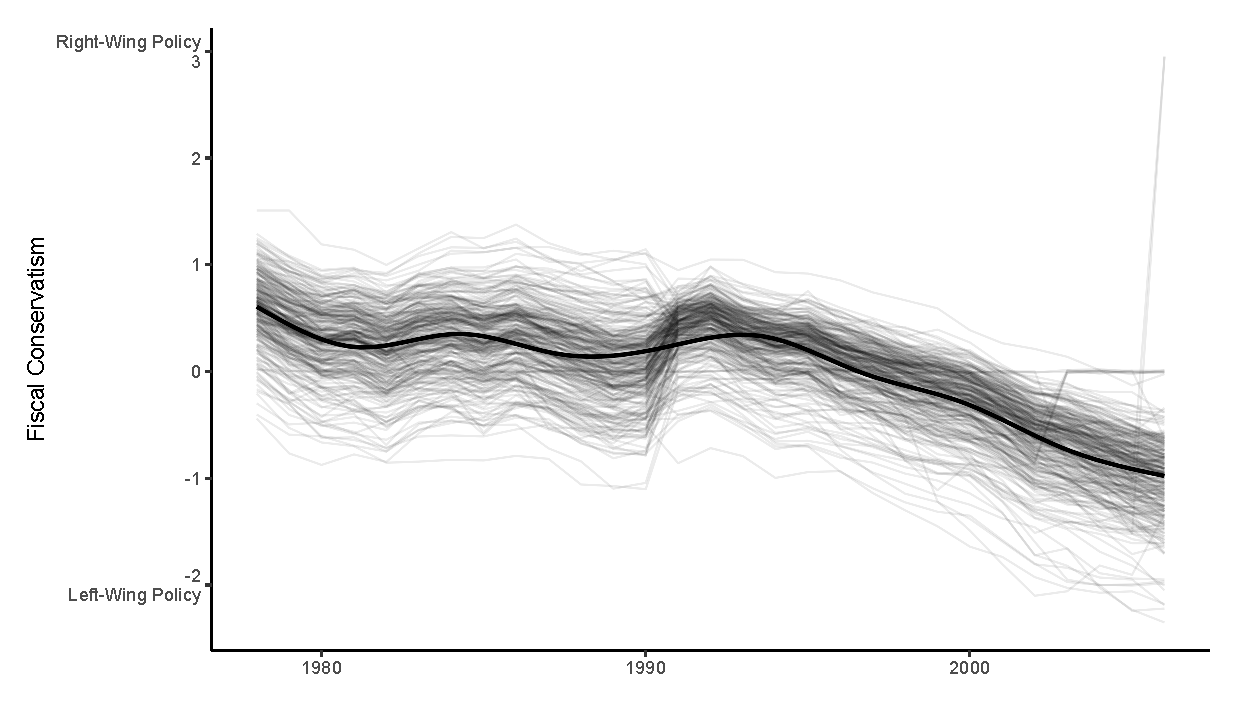
\includegraphics[width=1\textwidth]{fiscal_TimeSeries.eps}
	\caption{Average Municipal Fiscal Policy Conservatism (dark line) and Municipal Fiscal Policy Conservatism for Individual Municipalities (grey lines) from 1978 to 2006.}
	\label{fig:timeline}
	

	
\end{figure}


\subsection*{Municipal Policy Preferences}

In order to find out whether municipal fiscal policy conservatism responds to the preferences of the electorate, we need to develop a measure of local policy preferences. In line with previous work on municipal responsiveness \cite[e.g.,][]{sances2017ideology,einstein2016pushing}, we measure local policy preferences indirectly by examining the net difference in electoral support for right-wing and left-wing parties in the municipality, inferring that municipal electorates that prefer conservative parties also prefer conservative fiscal policies. In particular, we look at the difference between support for the major center-right parties as well as the right wing populist parties (Venstre, Det Konservative Folkeparti, Fremskridstpartiet and Dansk Folkeparti) and the major center-left parties as well as the socialist parties (Socialdemokratiet, Radikale Venstre, Socialistisk Folkeparti, Venstresocialisterne, and Enhedslisten) at all municipal elections in the period under study. This gives us an estimate of local policy preferences in the years 1978, 1981, 1985, 1989, 1993, 1997 and 2001.

 Unlike previous studies, which have had to rely on support for conservative vis-á-vis liberal parties at national or regional elections \citep[e.g.,][]{hajnal2010or,einstein2016pushing}, we are able to look at municipal elections. This is potentially important, because citizens might differ in their policy views across domains \cite[for an argument along these lines, see]{abrams2012big}, and because the electorate at municipal elections are differently composed than electorates in national elections \citep{ansolabehere2015beyond}. In Appendix  \ref{validation}, we show that there is added value in using municipal rather than national election returns. In particular, we find that in a concurrent municipal and national election, net support for conservative parties is far from perfectly correlated (Pearsons R=0.56).
 
 It might have been preferable to have survey based estimates of citizens policy ideal points \citep[similar to the measure used by][]{tausanovitch2014representation}. However, doing so is not feasible, as survey data is too sparse, especially for the earlier part of the period we study. Instead, we carry out a validation of our measure in Appendix \ref{validation}, in which we find that there is a strong correlation between net support for conservative parties at municipal elections and citizens' responses to an ideology question, using some recent survey data.

Table \ref{tab:desc} presents descriptive statistics on some key features of the Danish municipalities. For the most central variables to our analysis, we show descriptives on the levels as well as their within-municipality changes. It is noteworthy that while within-municipality evolution in fiscal policy conservatism as well as electoral support for right-wing parties is much smaller than the differences across all municipalities, they do vary quite a bit within municipalities over time.


\begin{table}[!htbp] \centering 
	\caption{Descriptive Statistics} 
	\label{tab:desc} 
		\begin{tabular}{@{\extracolsep{5pt}}lccccc} 
			\\[-1.8ex]\hline 
			\hline \\[-1.8ex] 
			Statistic & \multicolumn{1}{c}{N} & \multicolumn{1}{c}{Mean} & \multicolumn{1}{c}{St. Dev.} & \multicolumn{1}{c}{Min} & \multicolumn{1}{c}{Max} \\ 
			\hline \\[-1.8ex] 
			Full Fiscal Scale & 1,908 & 0.153 & 0.455 & $-$1.803 & 1.509 \\ 
			Full Fiscal Scale (Within) & 1,908 & 0.000 & 0.347 & $-$1.591 & 0.930 \\ 
			Reduced Fiscal Scale & 1,908 & 0.215 & 0.986 & $-$3.380 & 3.045 \\ 
			Reduced Fiscal Scale (Within) & 1,908 & $-$0.000 & 0.708 & $-$2.809 & 2.211 \\ 
			Support for Right-Wing Parties & 1,908 & 0.061 & 0.213 & $-$0.613 & 0.655 \\ 
			Support for Right-Wing Parties (Within) & 1,908 & $-$0.000 & 0.113 & $-$0.527 & 0.777 \\ 
			Population Size (logged) & 1,908 & 9.367 & 0.744 & 7.726 & 12.566 \\ 
			Education & 819 & 14.536 & 5.464 & 6.800 & 44.100 \\ 
			Immigrants & 818 & 143.265 & 160.195 & 3.000 & 1,344.000 \\ 
			Unemployment & 1,092 & 8.526 & 3.459 & 2.200 & 23.000 \\ 
			\hline \\[-1.8ex] 
		\end{tabular} 
\end{table} 



\section*{Identifying Dynamic Responsiveness in Cities}


Figure \ref{fig:scatter} shows that the past changes in support for right-wing parties are related to future changes in fiscal conservatism (full measure), suggesting that municipal policy adjusts dynamically to changes in the municipal electorate's preferences. This is striking, as we have minimized concerns related to reverse causality by looking at the relationship between past changes in preferences and future changes in policy within each municipality. Interestingly, we identify a non-linearity, but this pattern is not robust to alternative specifications (i.e., it disappears in a two-way fixed effects model), so we do not want to make any firm interpretations of what this implies.


\begin{figure}[h]
	\centering
	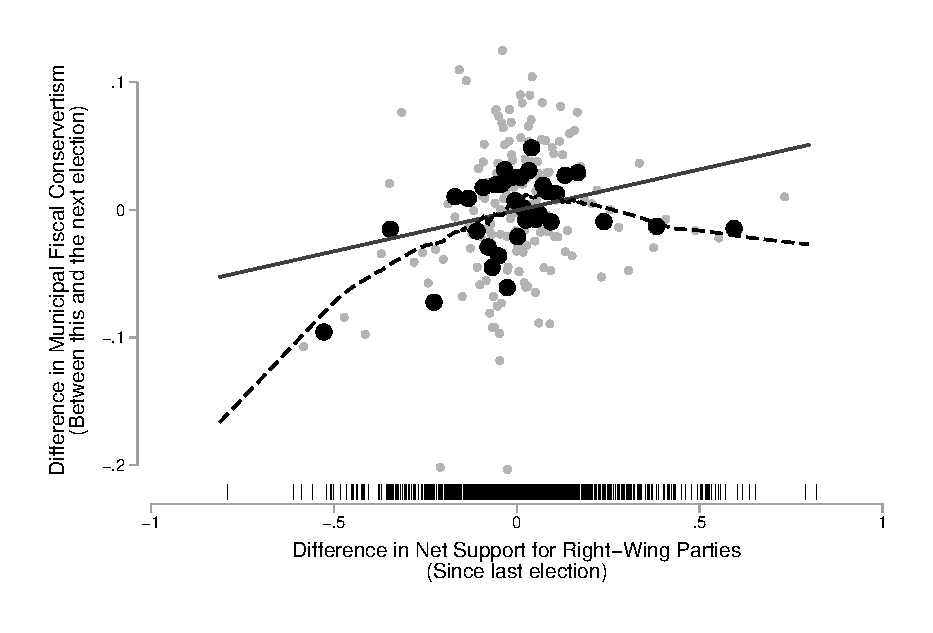
\includegraphics[scale = 0.8]{scatterplot.eps}
	\caption{Do Changes in Preferences Correlate with Future Changes in Policy? Both variables are trend adjusted (i.e., the year specific means are subtracted). Grey dots represent bins of ten observations, dark dots represent bins of 100  observations. The solid line is a linear fit (b$=0.046$, municipality clustured se$=0.019$) and the dashed line is a LOWESS smoother with a bandwidth of 0.4. The rugplot in the bottom of the graph represents the distribution of differences in the net support for right-wing parties. }
	\label{fig:scatter}
\end{figure}




Table \ref{tab:FourYearLead} presents the key estimate (i.e., the effect of changes in local policy preferences) from a pooled OLS regression, as well as from two types of difference-in-differences (diff-in-diff) models: a fixed effects and a first-difference model (both with time fixed effects). All models include a control for population size (logged), but the results do not depend on the inclusion of this covariate.  The  left panel uses the full measure of fiscal conservatism as the dependent variable whereas the right panel uses our reduced measure. Across all models, we find a statistically significant and positive effect.

The estimate from the pooled model is likely to be confounded by the socio-demographic make-up of the municipality. To the extent that this is stable over time and driven by common shocks, the difference between the estimates from the pooled and diff-in-diff models can be interpreted as removing the confounding effect of sticky socio-demographics. In our preferred fixed effects model, we estimate the effect to be roughly .12. This corresponds to 25 percent of a within-municipality standard deviation -- a substantive association. 


\begin{landscape}
	
	
	\begin{table}[!htbp] \centering 
		\caption{Effect of Electoral Support for Right-wing Parties on Municipal Conservatism 4 years later} 
		\label{tab:FourYearLead} 
		\begin{tabular}{@{\extracolsep{5pt}}lcccccccc} 
			\\[-1.8ex]\hline 
			\hline \\[-1.8ex] 
			& \multicolumn{8}{c}{\textit{Dependent variable:}} \\ 
			\cline{2-9} 
			\\[-1.8ex] & & \multicolumn{3}{c}{Full Fiscal Policy Scale} & 	&\multicolumn{3}{c}{Reduced Fiscal Policy Scale}   \\ 
			& Pooled & Fixed Effects & Diff Trend & First-Difference & Pooled & Fixed Effects & Diff Trend & First-Difference \\ 
			\\[-1.8ex] & (1) & (2) & (3) & (4) & (5) & (6) & (7) & (8)\\ 
			\hline \\[-1.8ex] 
			Right-Wing Vote Share & 0.416$^{**}$ & 0.129$^{**}$ & 0.145$^{**}$ & 0.065$^{**}$  & 1.110$^{**}$ & 0.317$^{**}$ & 0.335$^{**}$ & 0.144$^{**}$ \\ 
			& (0.083) & (0.044) & (0.048) & (0.025)  & (0.179) & (0.091) & (0.099) &  (0.055) \\ 
			Population Size (logged) & $-$0.097$^{**}$ & $-$0.711$^{**}$ &  & $-$0.596$^{**}$  & $-$0.180$^{**}$ & $-$1.197$^{**}$ &  & $-$0.977$^{*}$ \\ 
			& (0.022) & (0.202) &  & (0.178)  & (0.051) & (0.407) &  &  (0.387) \\ 
			Constant & 0.802$^{**}$ &  &  & $-$0.010 & 1.454$^{**}$ &  &  & $-$0.070$^{**}$ \\ 
			& (0.213) &  &  & (0.009) & (0.488) &  &  & (0.021) \\ 
			\hline \\[-1.8ex] 
			Municipality FE? & No & Yes & Yes & No & No & Yes & Yes & No \\ 
			Year FE? & No & Yes & Yes & Yes & No & Yes & Yes & Yes \\ 
			Year X Region FE? & No & No & Yes & No & No & No & Yes & No \\ 
			Four-Year Differenced? & No & No & No & Yes & No & No & No & Yes \\ 
			Observations & 1,908 & 1,908 & 1,908 & 1,633 & 1,908 & 1,908 & 1,908 & 1,633 \\ 
			\hline 
			\hline \\[-1.8ex] 
			\multicolumn{9}{p{25 cm}}{\emph{Note: Unstandardized OLS coefficients. Beck-Katz standard errors in parentheses in first-difference models, Arellano-White standard errors with clustering on municipality level used in the remaining models to correct for temporal autocorrelation. $^{*}$, and $^{**}$ indicate statistical significance at the 5 and 1 percent levels, respectively. Differences in the coefficients between panels are driven by a larger standard deviation in the reduced measure. See Appendix \ref{item} for results using the individual policy indicators.}} \\
		\end{tabular} 
	\end{table}
	
\end{landscape}

While the notion of fiscal policy conservatism can seem highly abstract, changes in our measure arise from fluctuations in municipal spending on particular public services, and how this spending is financed. All of which has real consequences for the citizens of a given municipality. An increase in overall conservatism of the magnitude estimated in the fixed effects model (column 2) is expected to be made up of reductions amounting to 13 and 11 percent of a standard deviation in income and property taxes, respectively, 17 percent of a standard deviation in spending per pupils in public schools, 9 percent of a standard deviation in the prevalence of public housing, 11 percent of a standard deviation in the number of public employees, and 23 percent of a standard deviation in overall spending per capita.\footnote{We arrive at these estimates by using the correlation between each item and the overall measure of fiscal policy conservatism. The full list of correlations is presented in Appendix \ref{estimation}.} These results indicate that when citizens change their preferences, it is likely to have notable real-world consequences for municipal fiscal policy and -- by extension -- the provision of specific local public services. 

\subsection*{Exploring the Identifying Assumption}
The identifying assumption in our diff-in-diff models is that trends in the dependent variable (policy) are independent of selection into the independent variable (preferences). Importantly, if voters became \emph{more conservative} as a result of changes in policy \cite[cf.][]{lenz2013follow}, then this assumption will be violated.

While we cannot test the identifying parallel trends assumption directly, we can see whether trends in the dependent variable are similar before municipalities "select into" different preferences.  To do this, we regress past levels of policy conservatism on current levels of net support for conservative parties using our two-way fixed effect set-up. The resulting effect is negligible and statistically insignificant, suggesting that trends in policy are parallel across municipalities that become more and municipalities that become less conservative  (see Figure \ref{fig:LongRun}). To  bolster this analysis further,  we show in Appendix \ref{granger} that past changes in municipal policy is unrelated with future changes in electoral support for right-wing parties.


Beyond this test,  we estimate a more restrictive model, where we interact the time fixed effects with a series of 13 regional dummies\footnote{These correspond to  13 regional governments (\textit{amter}) which were responsible for, among other things, health care in the period we study.} as well as population size. This allows municipalities to be on separate time trends depending on both region (semi-parametrically) and population size (log-linearly). Importantly, this strategy should deal with the confounding effect of the socio-demographic make-up of the municipalities: If there were certain time-specific regional shocks to, for instance, unemployment, which might affect both preferences and policy, then these will be removed in this model. As can be seen from Figure \ref{fig:FourYearLead}, estimating this more restrictive model does not change our results. If anything, the point estimate increases.

To make sure that there is no remaining bias because of socio-demographic factors, we include data on education, unemployment rate and the number of non-western immigrants in the municipality. Since these variables are only available after 1993, and there is a substantial trend in municipal policy (cf. Appendix \ref{descriptives}), simply including them in our model would bias our results by censoring the dependent variable. Instead, we follow \citep{pei2018poorly} and regress electoral support for right-wing parties on our three socio-demographic predictors. As we show in Appendix \ref{balance}, the correlations between within-municipality changes in socio-demographic factors and support for right-wing parties are very small and statistically insignificant. This suggests that these important socio-demographic factors are not driving our results, as right-wing and left-wing municipalities are balanced on these socio-demographic factors once we include fixed effects for time and year. The absence of a partial correlation with unemployment is especially noteworthy, as it is a strong indicator of whether a municipality is hit particularly hard by a temporary economic shock, which could feasibly drive both preferences and policy.

Taken together, these auxiliary analyses suggest that our identifying assumption is met, implying that we have a plausibly unbiased estimate of the effect of municipal policy preferences on municipal policy.

\subsection*{How Dynamic is Dynamic Responsiveness?}

To examine the temporal dynamics of responsiveness, figure \ref{fig:LongRun} reports the estimated effect of changes in net support for conservative parties on municipal fiscal policy conservatism over time. In panel A, we look at the short- and long-term effects of changes in municipal policy preferences on the policy adopted by the municipality. This analysis reveals that it takes some time for policy to respond. There is only a small effect one year after local policy preferences change and the largest effect is after four years. The effect is detactable up to eight years later. One reason for this long-term effect is probably that once policy shifts, it typically does not naturally revert back to it's starting point, but needs to be actively changed back \citep[e.g.,][]{baumgartner2009punctuated}. In Panel B we allow the effect of voter preferences on policy four years into the future to vary across time by including random slopes by year. The results show that municipal policy responsiveness is relatively stable across our period of study. Preferences do not seem to matter more or less as time goes by.

\begin{figure}[htbp]
	\centering
	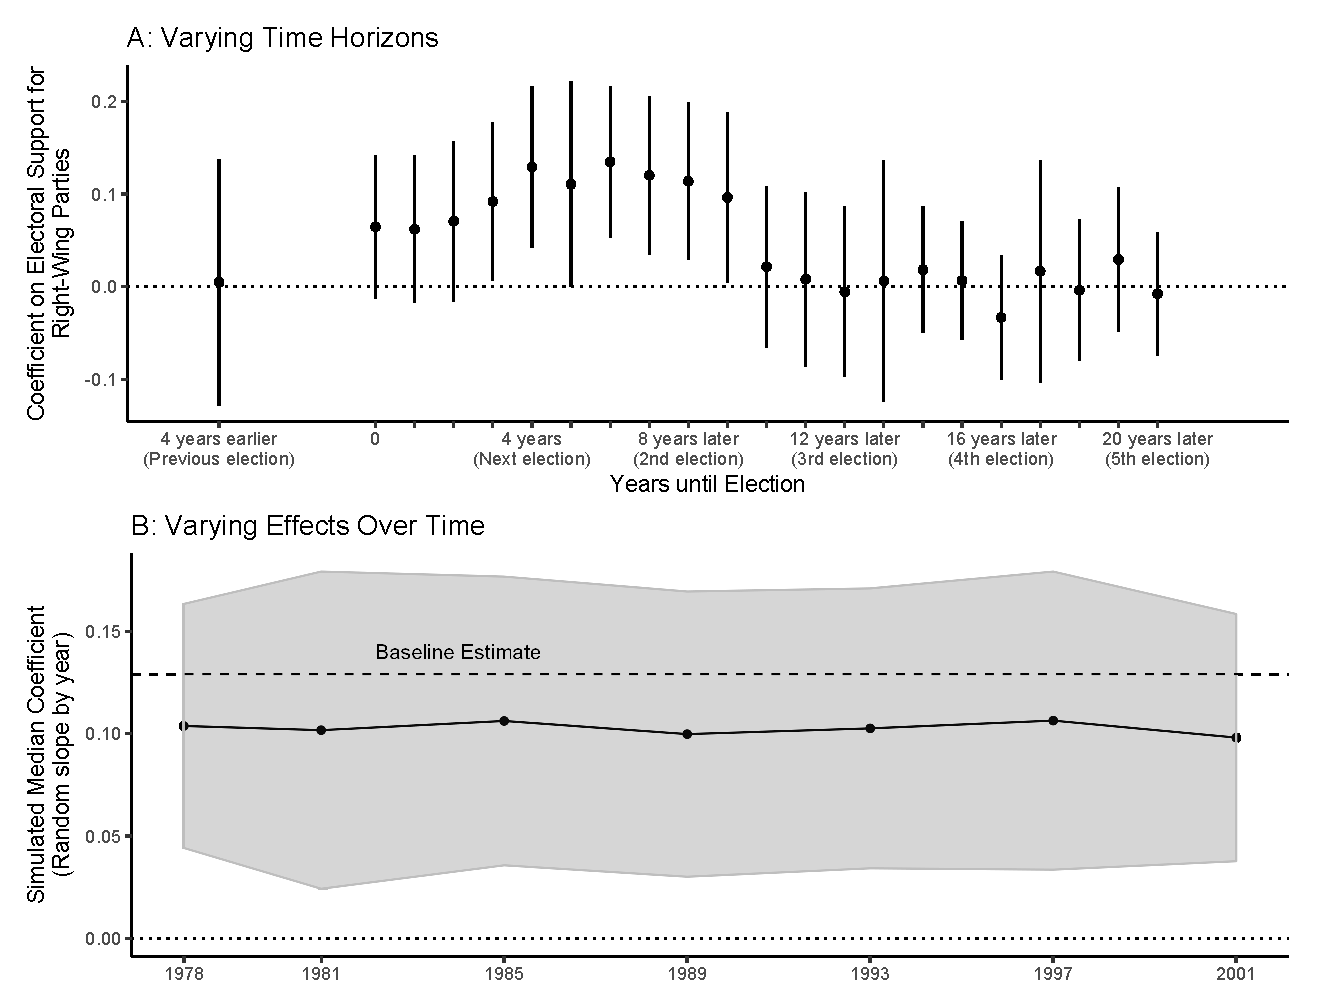
\includegraphics[scale = .6]{EffectsVsTime.eps}
	\caption{Effects of Local Policy Preferences Over Time. All models include two-way fixed effects with control for population size. Panel A: Black points represent the effect of net electoral support for conservative parties with different leads. Black lines are 95 percent CIs based on Arellano-White robust standard errors clustered on municipalities. Panel B: Points are estimates of random slopes by year with a lagged dependent variable to deal with autocorrelation. Shaded area is a 95 percent CI from the relevant percentiles of a bootstrapped distribution.}
	\label{fig:LongRun}
\end{figure}








\section*{Conclusion}

In this study, we have shown that municipal government is dynamically responsive to demands from citizens -- when more citizens express that they want more right-wing policy, policy responds; a result that was robust to a number of demanding specifications. Importantly, by using a more detailed and comprehensive measure of municipal policy, we were able to link past changes in preferences to future changes in policy, sidestepping potential concerns related to reverse causality. 

Even so, there are several outstanding questions. For one, we know little about why municipalities respond to citizen preferences. In Appendix \ref{mechanism}, we present some evidence to suggest that the effect is \textit{not} mediated by which party controls the municipal administration. However, this evidence is far from conclusive. Further, while we identify some dynamic responsiveness, it is hard to say whether this is adequate (or perhaps too much) from a normative democratic perspective.

Our study contributes directly to the literature on responsiveness \citep{tausanovitch2014representation}, and more broadly the empirical study of whether voters are able constrain the decision-making of political elites \citep{berry2009imperfect}. In particular, our study suggests that if you give voters an opportunity to express their preferences at municipal elections, they are able to use it to direct policy, substantially constraining local policy-makers.





\onehalfspacing
\bibliographystyle{apa}
\bibliography{library}

\clearpage

\renewcommand{\thesubsection}{\Alph{subsection}}
\renewcommand{\thetable}{\Alph{subsection}\arabic{table}}
\renewcommand{\thefigure}{\Alph{subsection}\arabic{figure}}


\end{document}

